% !TEX program = pdflatex
% Build: run pdflatex twice, or use `latexmk -pdf main.tex`
\documentclass[journal]{IEEEtran}

\usepackage[T1]{fontenc}
\usepackage{graphicx}
\usepackage{cite}
\usepackage{amsmath,amssymb}
\usepackage{booktabs}
\usepackage{xcolor}
\usepackage{array}
\usepackage{float}
\usepackage{tikz}
\usepackage{algorithm}
\usepackage{algorithmic}
\usetikzlibrary{positioning,fit}
\usepackage[hidelinks,hypertexnames=false]{hyperref}

\pagestyle{empty}

\DeclareGraphicsExtensions{.pdf,.png,.jpg,.jpeg}
\graphicspath{{../results/plots/}}

% Micro-spacing adjustments for page budget optimization
\setlength{\abovecaptionskip}{3pt}
\setlength{\belowcaptionskip}{3pt}
\setlength{\floatsep}{5pt plus 2pt minus 2pt}
\setlength{\textfloatsep}{5pt plus 2pt minus 2pt}
\setlength{\intextsep}{5pt plus 2pt minus 2pt}
\setlength{\parskip}{0pt}
\setlength{\abovedisplayskip}{3pt plus 1pt minus 1pt}
\setlength{\belowdisplayskip}{3pt plus 1pt minus 1pt}
\setlength{\abovedisplayshortskip}{0pt plus 1pt}
\setlength{\belowdisplayshortskip}{2pt plus 1pt minus 1pt}

% Title candidates (V5 revision):
% 1. Edge-AI Severity Regression and Asymmetric Loss for Controlled PV Electroluminescence Benchmarking and SCADA Alerting [APPLIED]
% 2. Safety-Aware EL Severity Regression on Edge Hardware with MQTT/PostgreSQL Maintenance Alerting: A Controlled Benchmark Study
% 3. Proof-of-Concept Edge-to-SCADA Pipeline for PV Electroluminescence Severity Regression with Asymmetric Huber Loss

\title{Edge-AI Severity Regression and Asymmetric Loss for Controlled PV Electroluminescence Benchmarking and SCADA Alerting}

\author{Wassim R. Hachemi\\
\textit{Department of Electronics, Faculty of Electrical Engineering}\\
\textit{University of Sciences and Technology Houari Boumediene (USTHB)}\\
Algiers, Algeria\\
wrhachemi@gmail.com}

\begin{document}

\maketitle
\thispagestyle{empty}

\begin{abstract}
This manuscript reports a controlled benchmark study that combines continuous EL severity regression, a Safety-Aware Asymmetric Huber Loss (SAHL) objective, Raspberry Pi ONNX deployment, and MQTT/Node-RED/PostgreSQL alerting on laboratory electroluminescence (EL) data. The work integrates known elements---cost-sensitive regression, edge inference, and auditable database-layer alert logic---into a bounded PV maintenance workflow rather than demonstrating field-validated autonomous inspection. Relative to an MSE baseline, SAHL at $\lambda=1.5$ yields modest multi-seed gains: critical recall rises from $0.784 \pm 0.048$ to $0.806 \pm 0.046$ (pred $\ge 0.6$, target $\ge 0.8$), MAE falls from $0.1959 \pm 0.0037$ to $0.1700 \pm 0.0047$, and F1 remains comparable ($0.756 \pm 0.013$ vs.\ $0.757 \pm 0.032$) at $\tau=0.65$. A multi-seed weight ablation across $\lambda \in \{1.0, 1.5, 2.5, 5.0\}$ shows no single weight dominates all metrics: 1.0$\times$ gives the strongest balanced F1 and precision, 1.5$\times$ gives the lowest MAE, 2.5$\times$ improves recall and critical recall at precision cost, and 5.0$\times$ is unstable. Weight selection therefore depends on operational objectives. A sustained Raspberry Pi 4 benchmark over 1,588 measured inferences reports ONNX latency of $190.32 \pm 27.93$ ms (median 177.63 ms, P95 238.77 ms), throughput of 5.25 FPS, and peak RSS of 128.98 MB. Full-module outdoor validation remains future work.
\end{abstract}

\begin{IEEEkeywords}
photovoltaic inspection, electroluminescence, severity regression, Safety-Aware Asymmetric Huber Loss, edge AI, ONNX, MQTT, Node-RED, predictive maintenance
\end{IEEEkeywords}

\section{Introduction}
PV operators need defect-screening workflows that detect severe degradation early while remaining usable on constrained edge hardware. We validate a cyber-physical inspection loop on controlled benchmark data, not on field deployment evidence.
Prior studies often evaluate model accuracy, edge deployment, and maintenance operations separately; this work examines these layers as one reproducible predictive-maintenance pipeline.

\subsection{Controlled EL Imaging Context and Scope}
The ZAE Bayern data are controlled, cell-level laboratory EL images. This setting supports method validation but does not represent full-module outdoor operation. Field factors such as thermal drift, dust accumulation, and long-term sensor aging are outside the present scope.

\subsection{Research Gap: Integrated Maintenance Intelligence Pipeline}
Existing literature offers fragmented progress: (i) EL defect recognition with high laboratory accuracy \cite{BuerhopLutz2018,Deitsch2019,Deitsch2021}, (ii) UAV-based thermal imaging for PV surveying \cite{Liao2022}, and (iii) IoT telemetry for remote monitoring \cite{Kunaifi2020,Kaswan2021}. However, practical predictive maintenance requires these elements to operate jointly: continuous severity estimation, maintenance-aware regression objectives, constrained edge execution, and auditable SCADA-linked alert management. Standard regression objectives such as MSE are also not explicitly aligned with maintenance risk asymmetry in high-severity regions. This paper develops a controlled, end-to-end workflow that integrates physically motivated acquisition assumptions, safety-aware regression, and database-governed operational alerting. UAV-based PV inspection and acquisition are treated as motivating context rather than as the sole scientific contribution.

\subsection{List of Contributions}
The principal contributions are:
\begin{enumerate}
\item \textbf{Continuous EL Defect Regression:} We formulate EL defect estimation as continuous severity regression over $[0,1]$ to preserve ranking granularity for maintenance prioritization.
\item \textbf{Safety-Aware Asymmetric Huber Loss (SAHL):} We apply an asymmetric Huber objective with tunable penalty $\lambda$ for critical underestimation, encoding operational risk asymmetry as an operating-policy parameter rather than a fixed optimum.
\item \textbf{Sustained Edge Benchmarking:} We report sustained Raspberry Pi 4 execution behavior over repeated loops, including latency distribution and memory observations.
\item \textbf{Predictive SCADA Integration:} We connect edge inference to MQTT, Node-RED, and PostgreSQL trigger logic so alert-state transitions are auditable and support longitudinal maintenance analytics.
\end{enumerate}
The asymmetry factor $\lambda$ is a tunable operating-policy knob; this study does not identify one universally optimal weight.

\section{Related Work}
EL-based PV diagnostics are well established for identifying micro-cracks and electrically inactive regions. Foundational EL benchmarks and cell-level pipelines have been formalized through dataset curation, defect classification, and robust cell segmentation \cite{BuerhopLutz2018,Deitsch2019,Deitsch2021}. Many published models still reduce the decision space to binary labels, limiting triage depth \cite{Kunaifi2020,Ziegler2022}. UAV-based thermal imaging enables broad spatial coverage of photovoltaic systems \cite{Liao2022}. Weighted objectives are common in classification \cite{Tan2020}. Edge deployment via efficient architectures and ONNX interoperability supports low-power inference \cite{He2016,Sandler2018,Cyphers2020}. Recent work explores IoT-enabled robotic inspection \cite{Kandil2024}, TinyML on climbing robots \cite{Lin2024,Lin2025}, SCADA-centered predictive maintenance \cite{Syamsuddin2024}, and advanced EL classification \cite{Ebied2025}. This study contributes an integrated, controlled proof-of-concept implementation that combines continuous severity regression, asymmetric risk encoding via SAHL, auditable database-layer alert logic, and a bounded edge-to-SCADA maintenance workflow. The framework formulates continuous severity regression and encodes maintenance risk asymmetry directly in the objective, then connects this inference layer to a trigger-governed telemetry stack (MQTT + Node-RED + PostgreSQL) so model outputs become auditable state transitions rather than standalone scores.

\section{Proposed Systems Architecture}\label{sec:architecture}

\subsection{Proposed Kinematic Framework and Data-Flow}
This manuscript models a proposed crawler-mounted optical subsystem intended to mitigate blur in long-exposure drone EL capture; hardware behavior is treated as a theoretical kinematic design target rather than validated field performance. Targeted tolerances include sub-millimeter relative displacement during the 15-second exposure window and repeatable panel registration across sequential capture points. The key systems argument is that acquisition stability constrains edge-model feasibility: as blur variance increases, required model capacity and post-processing complexity increase, pushing memory and latency demand beyond practical embedded budgets. A stable optical reference frame can therefore reduce downstream computational burden and support deterministic inference cadence in the proposed design.

\begin{figure*}[!t]
\centering
\resizebox{\textwidth}{!}{%
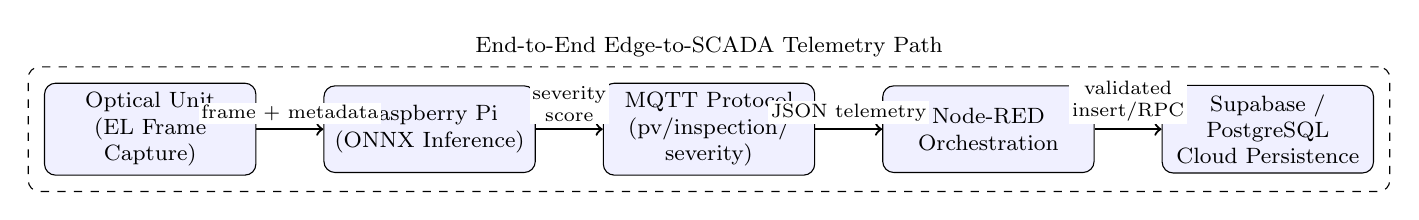
\begin{tikzpicture}[
  node distance=0.85cm,
  font=\footnotesize,
  block/.style={draw, rounded corners, align=center, minimum height=1.1cm, text width=2.45cm, fill=blue!6},
  arrow/.style={->, thick}
]
\node[block] (optical) {Optical Unit\\(EL Frame Capture)};
\node[block, right=of optical] (pi) {Raspberry Pi\\(ONNX Inference)};
\node[block, right=of pi] (mqtt) {MQTT Protocol\\(pv/inspection/\\severity)};
\node[block, right=of mqtt] (nodered) {Node-RED\\Orchestration};
\node[block, right=of nodered] (supabase) {Supabase / PostgreSQL\\Cloud Persistence};

\draw[arrow] (optical) -- node[midway, above=1.5pt, font=\scriptsize, fill=white, inner sep=1pt]{frame + metadata} (pi);
\draw[arrow] (pi) -- node[midway, above=1.5pt, align=center, font=\scriptsize, fill=white, inner sep=1pt]{severity\\score} (mqtt);
\draw[arrow] (mqtt) -- node[midway, above=1.5pt, font=\scriptsize, fill=white, inner sep=1pt]{JSON telemetry} (nodered);
\draw[arrow] (nodered) -- node[midway, above=1.5pt, align=center, font=\scriptsize, fill=white, inner sep=1pt]{validated\\insert/RPC} (supabase);

\node[draw, dashed, rounded corners, fit=(optical)(supabase), inner sep=0.2cm, label={[align=center]above:End-to-End Edge-to-SCADA Telemetry Path}] {};
\end{tikzpicture}%
}
\caption{System block diagram: Optical Unit $\rightarrow$ Raspberry Pi (ONNX Inference) $\rightarrow$ MQTT Protocol $\rightarrow$ Node-RED Orchestration $\rightarrow$ Supabase/PostgreSQL Cloud Persistence.}
\label{fig:system_block}
\end{figure*}

\subsection{Edge-to-Cloud Telemetry Orchestration}
At runtime, each EL frame is transformed into a severity score $s\in[0,1]$ and packaged with panel, pad, timestamp, and model metadata. MQTT transport decouples edge compute from cloud persistence and enables asynchronous retry under intermittent connectivity. Node-RED performs schema validation, payload normalization, and insertion/RPC invocation toward Supabase PostgreSQL. This design limits business logic embedded in edge firmware. If edge connectivity degrades, the acquisition and inference loop can continue in degraded mode while preserving local records for delayed publication, and policy updates can be deployed in Node-RED and SQL layers without retraining the model.

\subsection{Predictive Database Schema and Logic}
The cloud persistence layer uses relational entities for assets, thresholds, inspections, and alerts. Predictive logic is implemented in SQL functions and triggers, enabling deterministic state transitions from raw severity sequences. The trigger policy combines threshold exceedance and short-horizon slope to open, maintain, or resolve alerts, keeping decision logic transparent, auditable, and versionable in migration scripts. The alert policy evaluates three principal branches: a critical-threshold branch that opens alerts immediately, a trend branch that triggers when short-horizon slope indicates deterioration, and a recovery branch that resolves alerts when severity returns below recovery limits.

\section{Safety-Critical AI Methodology}\label{sec:methodology}

\subsection{Dataset and Labeling Strategy}
We use the public ZAE Bayern EL dataset. The original ZAE Bayern cell-level discrete probability labels (0.0, 0.33, 0.67, 1.0) were utilized directly as continuous regression targets. A separate integer bucketization strategy was applied to these labels purely to ensure balanced, stratified cross-validation splits during training.

This formulation preserves defect ordering and supports threshold tuning for operational policy.

\subsection{Noise Analysis for Long-Exposure EL Frames}
Long-exposure EL capture can be modeled as
\begin{equation}
I_{obs}(x,y)=I_{EL}(x,y)+n_g(x,y)+n_t(x,y)+n_i(x,y),
\label{eq:noise_model}
\end{equation}
where $n_g$ is approximately Gaussian read noise, $n_t$ denotes thermally driven dark-current variation, and $n_i$ represents impulse outliers (hot pixels). For hot pixels, $n_i$ is sparse with high amplitude relative to local neighborhood statistics:
\begin{equation}
\Pr\{|n_i|\gg \sigma_g\} \ll 1, \quad \text{but } |n_i| \text{ is large when present.}
\label{eq:impulse_model}
\end{equation}
A linear filter (for example mean filtering) spreads impulse artifacts into neighboring pixels, reducing edge contrast in fine crack structures. By contrast, the 5$\times$5 median filter
\begin{equation}
\hat{I}(x,y)=\operatorname{median}\{I_{obs}(u,v):(u,v)\in\mathcal{N}_{5\times5}(x,y)\}
\label{eq:median}
\end{equation}
rejects sparse outliers while preserving discontinuities associated with micro-crack boundaries. This order-statistic behavior is particularly useful for EL defect morphology where spatially thin crack lines carry high diagnostic value.

\subsection{Model and Training Protocol}
A ResNet18 backbone with sigmoid regression head is used for severity prediction \cite{He2016}:
\begin{equation}
\hat{y}=\sigma(z)=\frac{1}{1+e^{-z}},\quad \hat{y}\in(0,1).
\label{eq:sigmoid_output}
\end{equation}
Training follows a warmup-to-unfreeze strategy: initial head adaptation, followed by full-network fine-tuning at reduced learning rate. This protocol stabilizes transfer on moderate-size EL datasets while preserving high-level visual priors.

Data augmentation includes horizontal/vertical flips, mild rotation, and illumination jitter constrained to preserve crack topology. Augmentation is intentionally conservative to avoid generating synthetic artifacts that could blur defect boundaries.

\subsection{Safety-Aware Asymmetric Huber Loss (SAHL)}\label{sec:sahl}
Let $\Delta=\hat{y}-y$ and $\delta$ be the Huber transition parameter. SAHL is defined here as an application of cost-sensitive learning within an edge-constrained IoT pipeline. It is not introduced as a fundamentally new machine learning algorithm. Its form is
\begin{equation}
\mathcal{L}_{\mathrm{SAHL}}(\hat{y},y)=
\begin{cases}
\lambda\,\mathcal{H}_{\delta}(\Delta), & \text{if } y\ge 0.70\ \text{and}\ \hat{y}<0.70,\\
\mathcal{H}_{\delta}(\Delta), & \text{otherwise},
\end{cases}
\label{eq:sahl}
\end{equation}
with
\begin{equation}
\mathcal{H}_{\delta}(\Delta)=
\begin{cases}
\tfrac{1}{2}\Delta^2, & |\Delta|\le \delta,\\
\delta\left(|\Delta|-\tfrac{\delta}{2}\right), & |\Delta|>\delta.
\end{cases}
\label{eq:huber}
\end{equation}

Unlike standard quantile regression, which uniformly biases the median, or a globally weighted MSE, which can amplify noise across all severity bands, SAHL selectively targets the safety-critical region. The Huber component maintains robustness against annotation noise in the remaining distribution. Although the hard conditional boundary at $\hat{y} = 0.70$ creates a piecewise gradient, PyTorch's subgradient resolution via \texttt{torch.where} handles the transition natively. The warmup-to-unfreeze training protocol stabilized convergence across this boundary. We evaluate $\lambda \in \{1.0, 1.5, 2.5, 5.0\}$; illustrative figures and the MSE comparison in Table~\ref{tab:metrics} use V3.1 at $\lambda=1.5$.

\subsection{Operational Risk Minimization Perspective}
SAHL bridges machine learning and reliability engineering: the asymmetry encodes unequal consequence, where missing a severe defect creates higher downstream risk than issuing a conservative alert. This can be interpreted as minimizing expected operational cost
\begin{equation}
\mathbb{E}[C]=C_{FN}P(FN)+C_{FP}P(FP), \quad C_{FN}\gg C_{FP},
\label{eq:operational_cost}
\end{equation}
with SAHL reducing $P(FN)$ in the critical severity region by design.

In reliability terms, the loss can be interpreted as a proxy for asymmetric hazard exposure. False negatives delay intervention, effectively increasing expected exposure interval before maintenance. SAHL reduces this delay by shifting model sensitivity in the high-risk region. The loss function is a design instrument that encodes maintenance philosophy directly into gradient updates.

\subsection{Threshold Selection and Calibration}
Although SAHL improves score distribution in critical regions, final operational behavior is controlled by threshold calibration. We select $\tau=0.65$ from F1-threshold analysis while checking that critical recall remains high enough for preventive maintenance policy. This two-stage strategy (loss shaping + threshold tuning) avoids overfitting operational behavior to a single scalar objective. Threshold stability across seeds and sites was not fully characterized in this study; Section~\ref{sec:results} reports results at this fixed operating point.

\subsection{Evaluation Protocol}
Evaluation is performed on held-out test data using both ranking metrics (AP, ROC-AUC) and policy metrics (precision/recall/F1 at operating threshold). We additionally inspect confusion matrices and error distributions to detect whether improvements are concentrated in high-severity zones. Critical recall is reported at pred $\ge 0.6$ and target $\ge 0.8$ unless otherwise noted.

\subsection{Edge Inference and Telemetry Procedure}
\begin{algorithm}[!t]
\caption{Edge-to-SCADA Telemetry Loop}
\label{alg:edge_scada}
\scriptsize
\begin{algorithmic}[1]
\STATE Initialize camera, ONNX session, MQTT client, and metadata context
\LOOP
\STATE Capture long-exposure EL frame and apply denoising/normalization
\STATE Run ONNX inference to obtain severity score $s\in[0,1]$
\STATE Assign operational status from threshold policy
\STATE Build payload with IDs, score, status, model version, and timestamp
\STATE Publish payload to \texttt{pv/inspection/severity}
\STATE Validate and persist inspection record through Node-RED
\STATE Execute SQL alert-state evaluation and refresh dashboard widgets
\ENDLOOP
\end{algorithmic}
\end{algorithm}
Algorithm~\ref{alg:edge_scada} summarizes the edge inference and telemetry handoff used to convert frame-level severity estimates into auditable SCADA alert transitions.

\section{Experimental Results}\label{sec:results}

\subsection{Comparative Metrics at Operating Threshold}
Table~\ref{tab:metrics} reports multi-seed mean $\pm$ standard deviation for MSE baseline (V1) and SAHL model V3.1 at $\lambda=1.5$ at $\tau=0.65$. Critical recall uses pred $\ge 0.6$ and target $\ge 0.8$. Weight tradeoffs across $\lambda$ are reported separately in Table~\ref{tab:ablation}.

\begin{table}[!t]
\centering
\caption{V1 (MSE) vs.\ V3.1 (SAHL 1.5$\times$) at $\tau=0.65$ (Mean $\pm$ Std over 3 seeds; critical recall at pred $\ge 0.6$, target $\ge 0.8$)}
\label{tab:metrics}
\begin{tabular}{lcc}
\toprule
Metric & V1 & V3.1 \\
\midrule
F1 @ $\tau$ & $0.756 \pm 0.013$ & $0.757 \pm 0.032$ \\
Precision @ $\tau$ & $0.856 \pm 0.021$ & $0.828 \pm 0.035$ \\
Recall @ $\tau$ & $0.677 \pm 0.032$ & $0.699 \pm 0.053$ \\
Critical Recall & $0.784 \pm 0.048$ & $0.806 \pm 0.046$ \\
MAE & $0.1959 \pm 0.0037$ & $0.1700 \pm 0.0047$ \\
\bottomrule
\end{tabular}
\end{table}

At $\tau=0.65$, V3.1 at $\lambda=1.5$ shows directionally favorable but modest gains over MSE: critical recall increases by 0.022 (0.784 to 0.806), MAE decreases by 0.026, and F1 remains comparable within reported variance. Precision decreases moderately. These claims apply only to this comparison setting; they do not imply a universally optimal asymmetry weight.

\subsection{Multi-Seed SAHL Weight Ablation}
Table~\ref{tab:ablation} summarizes a multi-seed ablation across four asymmetry weights. No single weight dominates all metrics. At 1.0$\times$, F1 ($0.774 \pm 0.008$) and precision ($0.854 \pm 0.065$) are strongest among evaluated settings. At 1.5$\times$, MAE is lowest ($0.1700 \pm 0.0047$). At 2.5$\times$, recall ($0.760 \pm 0.049$) and critical recall ($0.846 \pm 0.028$) improve relative to 1.0$\times$ and 1.5$\times$, but precision and MAE worsen. At 5.0$\times$, recall and critical recall rise further, but F1, precision, and MAE degrade sharply with high variance (for example, F1 $0.551 \pm 0.129$, MAE $0.4524 \pm 0.1821$), indicating an over-aggressive and unstable operating regime.

\begin{table*}[!t]
\centering
\caption{Multi-Seed SAHL Weight Ablation (Mean $\pm$ Std over seeds 42, 123, 2026; $\tau=0.65$; critical recall at pred $\ge 0.6$, target $\ge 0.8$)}
\label{tab:ablation}
\begin{tabular}{lccccc}
\toprule
Weight & F1 @ $\tau$ & Precision & Recall & Critical Recall & MAE \\
\midrule
1.0$\times$ & $0.774 \pm 0.008$ & $0.854 \pm 0.065$ & $0.712 \pm 0.042$ & $0.815 \pm 0.040$ & $0.1734 \pm 0.0125$ \\
1.5$\times$ & $0.757 \pm 0.032$ & $0.828 \pm 0.035$ & $0.699 \pm 0.053$ & $0.806 \pm 0.046$ & $0.1700 \pm 0.0047$ \\
2.5$\times$ & $0.758 \pm 0.020$ & $0.757 \pm 0.018$ & $0.760 \pm 0.049$ & $0.846 \pm 0.028$ & $0.1898 \pm 0.0122$ \\
5.0$\times$ & $0.551 \pm 0.129$ & $0.423 \pm 0.181$ & $0.896 \pm 0.098$ & $0.944 \pm 0.073$ & $0.4524 \pm 0.1821$ \\
\bottomrule
\end{tabular}
\end{table*}

Weight selection is therefore a policy choice. Operators prioritizing balanced threshold metrics may prefer 1.0$\times$; those prioritizing regression error may prefer 1.5$\times$; those prioritizing critical-case sensitivity may prefer 2.5$\times$ at the cost of precision and MAE. The 5.0$\times$ setting is not recommended as a default given its instability.

\subsection{Confusion Matrix and False-Negative Reduction}
In a single representative run at $\tau=0.65$, the confusion-matrix shift from 44 to 26 false negatives corresponds to a 41\% reduction in missed severe defects for V3.1 at $\lambda=1.5$ versus MSE. This figure is illustrative only and is not aggregated across seeds.

\begin{figure}[!t]
\centering
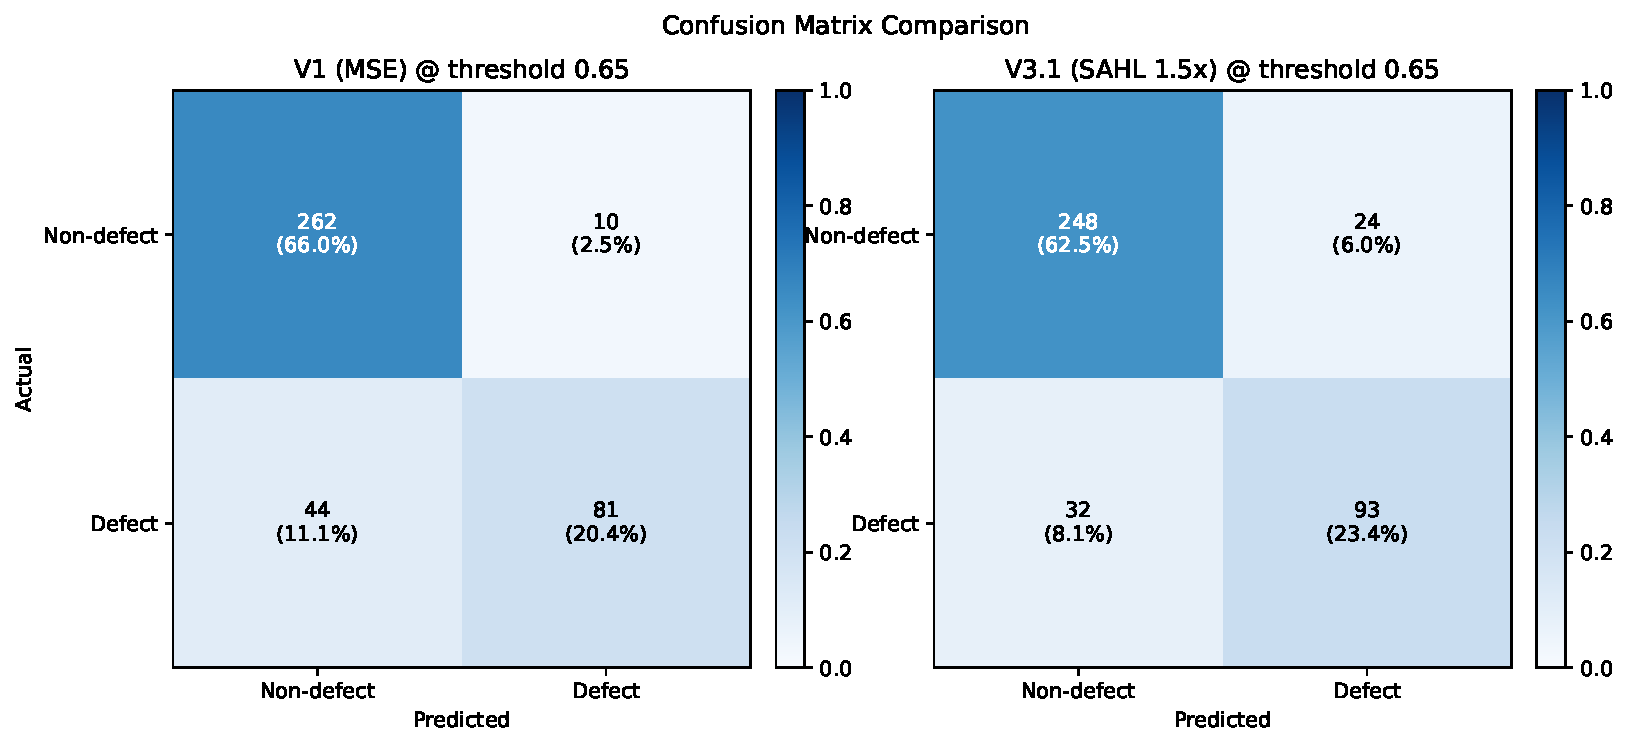
\includegraphics[width=0.85\linewidth]{confusion_matrices_at_operating_threshold.pdf}
\caption{Confusion matrices at $\tau=0.65$: V1 (MSE, left) vs.\ V3.1 (SAHL 1.5$\times$, illustrative configuration, right), showing false negatives reduced from 44 to 26 in this single run.}
\label{fig:confusion_matrix}
\end{figure}

\subsection{Precision-Recall and Threshold Behavior}
\begin{figure}[!t]
\centering
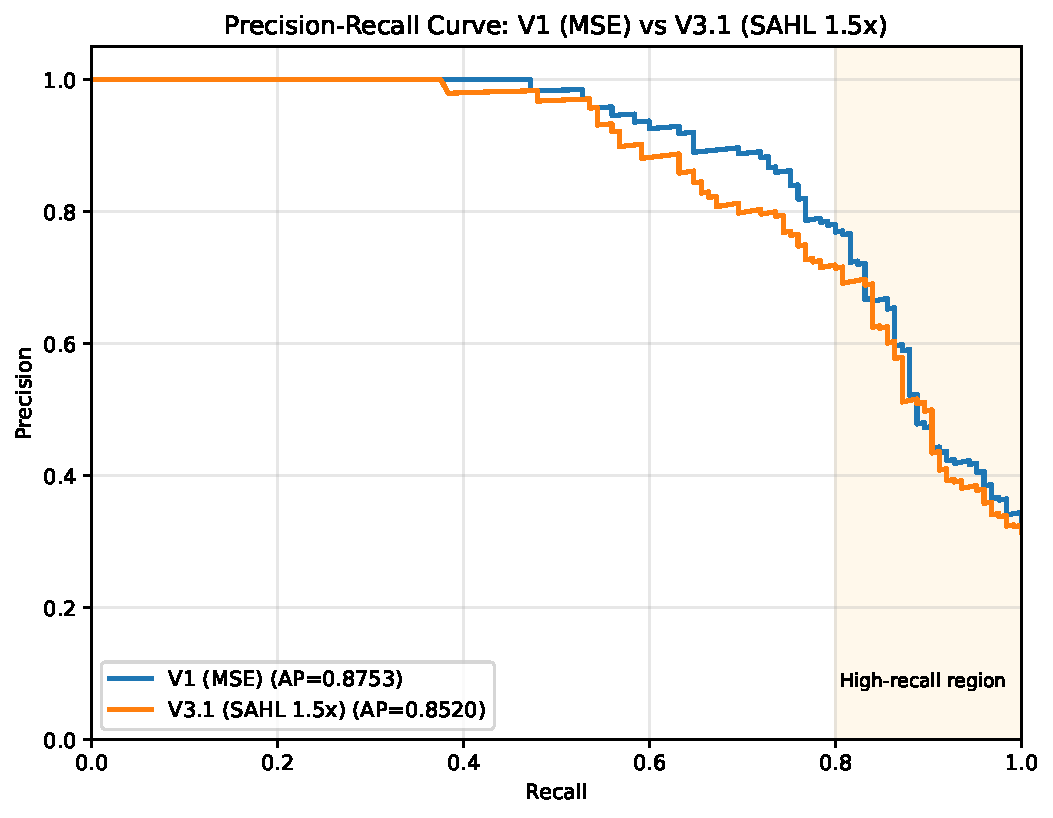
\includegraphics[width=0.85\linewidth]{pr_curve_v1_vs_v3_1.pdf}
\caption{Precision-recall comparison between V1 (MSE baseline) and V3.1 (SAHL 1.5$\times$, illustrative configuration).}
\label{fig:pr_curve}
\end{figure}

\begin{figure}[!tb]
\centering
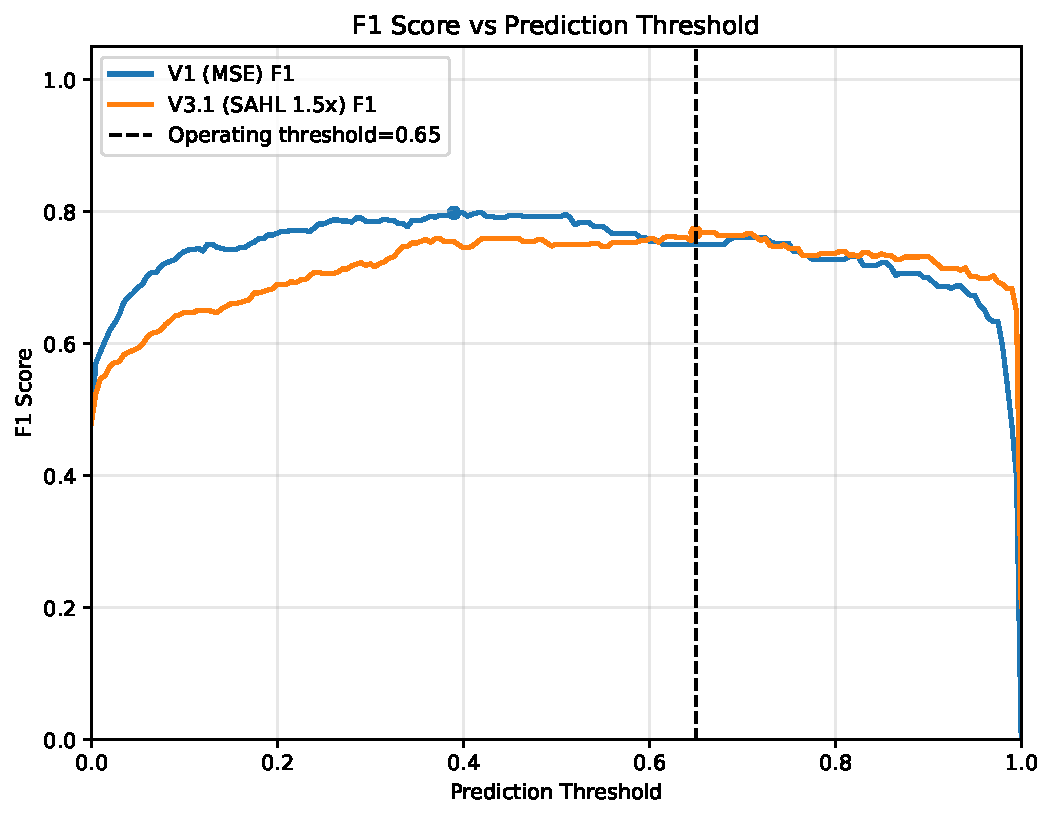
\includegraphics[width=0.85\linewidth]{f1_vs_threshold.pdf}
\caption{F1 versus decision threshold for V3.1 (SAHL 1.5$\times$, illustrative configuration) with operating point $\tau=0.65$ selected per Section~\ref{sec:methodology}.}
\label{fig:f1_vs_threshold}
\end{figure}

The precision-recall frontier indicates that SAHL at $\lambda=1.5$ favors higher-recall operating regimes at $\tau=0.65$. Figure~\ref{fig:f1_vs_threshold} shows how F1 varies with threshold; $\tau=0.65$ was chosen from this curve subject to critical-recall constraints. Threshold stability across seeds and alert-volume tradeoffs were not analyzed in this study and remain necessary next-step experiments.

\subsection{Error Distribution Analysis}
To complement threshold metrics, we inspect absolute regression error distributions. Figure~\ref{fig:error_dist} shows that SAHL maintains compact error mass near zero while reducing severe underestimation tails in high-risk regions.

\begin{figure}[!tb]
\centering
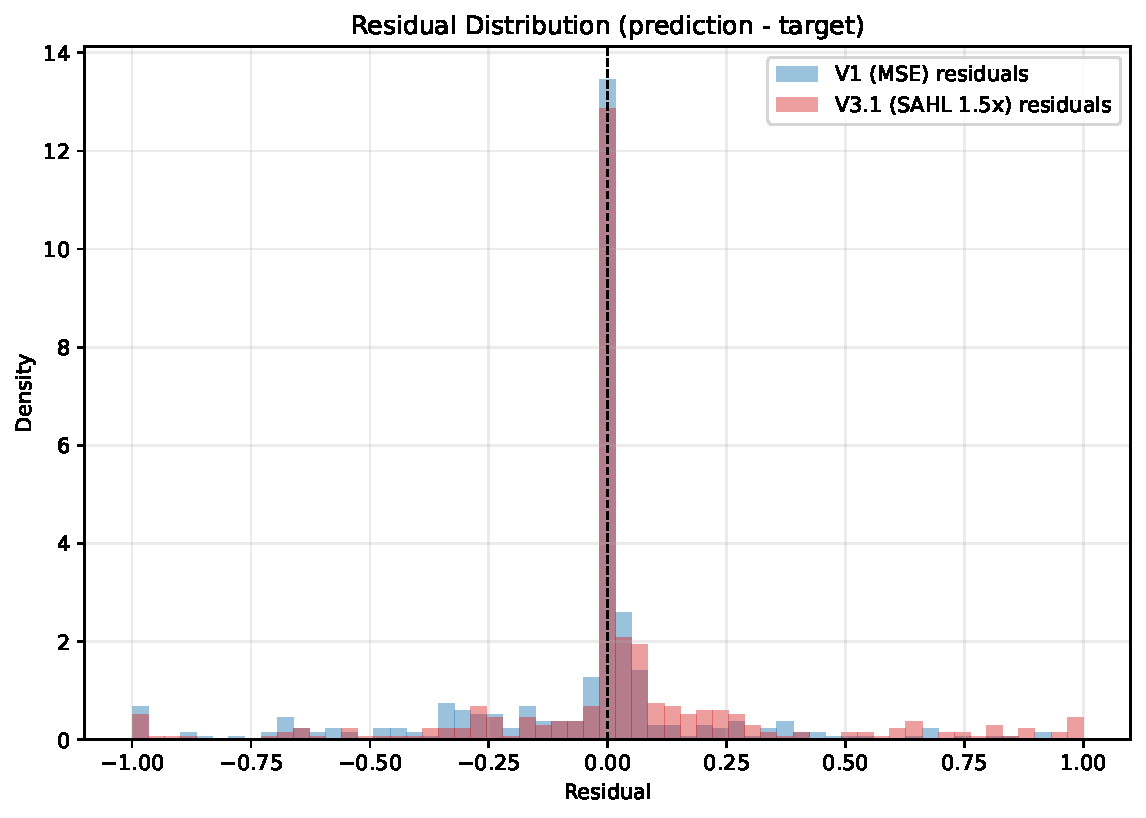
\includegraphics[width=0.85\linewidth]{error_distribution_comparison.pdf}
\caption{Absolute error distribution comparison between V1 (MSE baseline) and V3.1 (SAHL 1.5$\times$, illustrative configuration).}
\label{fig:error_dist}
\end{figure}

\subsection{Raspberry Pi Performance and Deployment Feasibility}
Table~\ref{tab:pi_summary} consolidates edge feasibility indicators for latency, throughput, and memory.

\begin{table}[!t]
\centering
\caption{Raspberry Pi 4 Sustained Performance Summary (V3.1 SAHL 1.5$\times$, ONNX, illustrative configuration)}
\label{tab:pi_summary}
\begin{tabular}{lc}
\toprule
Metric & Value \\
\midrule
Measured Inferences & 1,588 \\
Image Count / Loops / Warmups & 397 / 4 / 10 \\
ONNX Latency Mean $\pm$ Std (ms) & 190.32 $\pm$ 27.93 \\
ONNX Median Latency (ms) & 177.63 \\
ONNX P95 Latency (ms) & 238.77 \\
ONNX Throughput (FPS) & 5.25 \\
Peak RSS (MB) & 128.98 \\
\bottomrule
\end{tabular}
\end{table}

Observed memory behavior remained stable over the benchmark window, with RSS rising during model/session initialization and then remaining in a bounded range during sustained inference.

\subsection{Operational Implications}
Within this controlled benchmark setting, a safety-calibrated regression objective can improve prioritization for downstream inspection workflows. Defects with higher estimated severity can be surfaced earlier, while alert-state logic remains auditable in the persistence layer.

\begin{figure*}[!t]
\centering
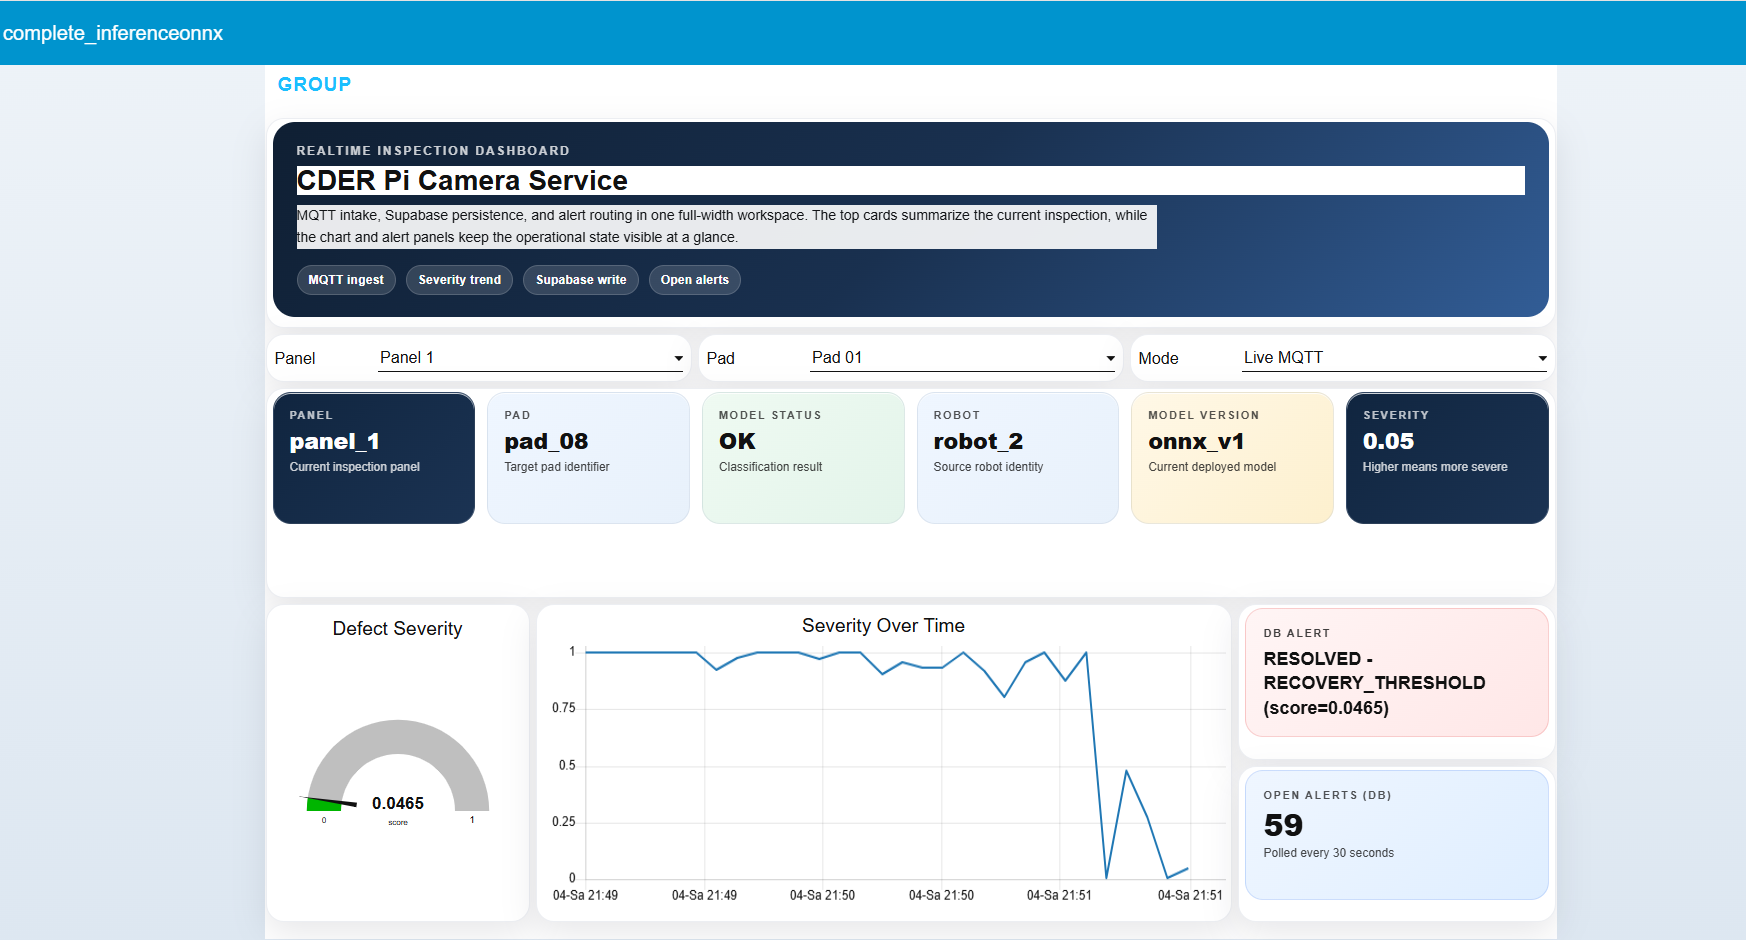
\includegraphics[width=0.55\linewidth]{dashboard_live.png}
\caption{Node-RED dashboard for severity tracking (V3.1 SAHL 1.5$\times$, illustrative configuration) and alert-state observability.}
\label{fig:nodered_dashboard}
\end{figure*}

\section{Discussion and Critical Analysis}\label{sec:discussion}

\subsection{Precision-Recall Trade-off in Safety-Critical Operations}
Table~\ref{tab:metrics} shows that V3.1 at $\lambda=1.5$ accepts a moderate precision decrease in exchange for higher recall and critical recall relative to MSE at $\tau=0.65$. In safety-critical maintenance, this trade-off is rational when false negatives carry substantially higher cost than false positives. The operating threshold reflects policy, not statistical optimality alone.

\subsection{Asymmetry Weight as Operational Control Knob}
Table~\ref{tab:ablation} shows no single $\lambda$ dominates all metrics. Higher weights reduce false-negative risk in the critical regime but increase alert burden, lower precision, and can destabilize regression error. Lower weights improve balanced F1 and precision but may under-weight severe misses. We do not recommend one universal default: 1.0$\times$ suits balanced threshold performance, 1.5$\times$ suits lowest MAE, 2.5$\times$ suits safety-first recall at higher precision cost. SAHL reshapes the trade-off surface among precision, recall, F1, MAE, and critical recall according to maintenance policy rather than yielding a globally optimal setting. The 5.0$\times$ setting illustrates diminishing returns and high variance and is not recommended as a default.

\subsection{Scope, Generalization, and Limitations}
Generalization across monocrystalline and polycrystalline modules depends on texture statistics, grain boundaries, and EL contrast characteristics. Because the ZAE corpus includes heterogeneous module appearances, the learned representation may transfer better than single-type training sets, though domain shift remains possible under site-specific optics and thermal conditions. These findings should therefore be interpreted as laboratory validation under controlled conditions rather than evidence of field-ready deployment. This study reports a proposed kinematic framework rather than field-validated mechanical deployment. The ablation uses three seeds and one operating threshold ($\tau=0.65$); weight choice should be interpreted as policy-sensitive rather than universal. Dataset-to-field transfer under environmental drift (dust, optics contamination, thermal gradients) is unvalidated. An exploratory out-of-distribution probe on 50 external EL images \cite{TheMakiran2026} was not statistically sufficient for formal generalization claims. Strong EL classification baselines, calibration analysis, and field validation remain future work. Periodic threshold review and version-controlled alert policies are advisable before any production rollout.

\section{Future Work}\label{sec:future}
Credible field validation requires staged deployment: shadow-mode logging, assisted operation with technician confirmation, and selective closed-loop alerting once metrics stabilize locally. Pilots should span heterogeneous sites to separate model limits from environmental confounders. Outdoor validation under thermal drift, dust, and sensor aging is essential before utility-scale claims. Extension of multi-seed ablation with threshold sweeps, calibration curves, and alert-volume analysis, together with ZAE-derived classification baselines and alternative cost-sensitive regression objectives, remain high-priority next steps.

\section{Conclusion}\label{sec:conclusion}
This controlled benchmark study presents an integrated predictive-maintenance framework combining continuous EL severity regression, a maintenance-oriented asymmetric Huber objective, Raspberry Pi ONNX edge inference, MQTT telemetry, Node-RED orchestration, and PostgreSQL trigger-governed alert logic within one reproducible edge-to-SCADA workflow. Multi-seed results show asymmetry tuning reshapes the maintenance-relevant trade-off surface rather than yielding one universally optimal weight. The principal value lies in operational integration and auditability of the complete pipeline, while empirical claims remain bounded to the present laboratory benchmark. Full-module outdoor validation remains future work.

\section*{ACKNOWLEDGMENTS}
The author acknowledges the physical space provided by the Centre de D\'eveloppement des \'Energies Renouvelables (CDER) during the initial observation phase of this project.

\textbf{AI Disclosure:} In accordance with IEEE policy 8.2.1.B.10, the author acknowledges the use of large language models (Google Gemini 3.1 Pro, OpenAI GPT-5.3) for literature synthesis, mathematical derivation verification, and structural polishing, as well as GitHub Copilot for code optimization. The author retains full accountability for the technical content, data integrity, and interpretations presented in this work.

\textbf{Data Availability:} Derived benchmark summaries, model-comparison metrics, dashboard artifacts, and the inference codebase used in this manuscript are publicly available at: \url{https://github.com/WRH-05/PV-Edge-SCADA}.

% Bibliography ordered by first citation appearance (required for IEEEtran + cite).
\begin{thebibliography}{99}

\bibitem{BuerhopLutz2018} C. Buerhop-Lutz, S. Deitsch, A. Maier, F. Gallwitz, S. Berger, B. Doll, J. Hauch, C. Camus, and C. J. Brabec, ``A benchmark for visual identification of defective solar cells in electroluminescence imagery,'' in \emph{Proc. Eur. PV Solar Energy Conf. Exhib. (EU PVSEC)}, 2018. doi: 10.4229/35thEUPVSEC20182018-5CV.3.15.

\bibitem{Deitsch2019} S. Deitsch, V. Christlein, S. Berger, C. Buerhop-Lutz, A. Maier, F. Gallwitz, and C. Riess, ``Automatic classification of defective photovoltaic module cells in electroluminescence images,'' \emph{Solar Energy}, vol. 185, pp. 455--468, 2019. doi: 10.1016/j.solener.2019.02.067.

\bibitem{Deitsch2021} S. Deitsch, C. Buerhop-Lutz, E. Sovetkin, A. Steland, A. Maier, F. Gallwitz, and C. Riess, ``Segmentation of photovoltaic module cells in uncalibrated electroluminescence images,'' \emph{Machine Vision and Applications}, vol. 32, no. 4, 2021. doi: 10.1007/s00138-021-01191-9.

\bibitem{Liao2022} K.-C. Liao, H.-Y. Wu, and H.-T. Wen, ``Using Drones for Thermal Imaging Photography and Building 3D Images to Analyze the Defects of Solar Modules,'' \emph{Inventions}, vol. 7, no. 3, p. 67, 2022, doi:10.3390/inventions7030067.

\bibitem{Kunaifi2020} K. Kunaifi, K. Otsuki, A. Phinikarides, N. Djordjevic, D. Sera, and R. Heylen, ``Advanced monitoring techniques for photovoltaic systems,'' \emph{Prog. Photovolt. Res. Appl.}, vol. 28, no. 7, pp. 629--644, 2020.

\bibitem{Kaswan2021} K. K. Kaswan, P. Singh, and H. Singh, ``Machine learning for photovoltaic fault diagnosis: A survey,'' \emph{Renew. Sustain. Energy Rev.}, vol. 145, p. 111103, 2021.

\bibitem{Ziegler2022} T. Ziegler, S. Wendt, C. Libal, and A. M\"uller, ``Deep learning for solar module defect detection,'' in \emph{Proc. IEEE Photovoltaic Specialists Conf.}, 2022, pp. 1--6.

\bibitem{Tan2020} M. Tan, R. Prapong, and Q. V. Le, ``EfficientNet: Rethinking model scaling for convolutional neural networks,'' in \emph{Proc. Int. Conf. Mach. Learn.}, 2020, pp. 6105--6114.

\bibitem{He2016} K. He, X. Zhang, S. Ren, and J. Sun, ``Deep residual learning for image recognition,'' in \emph{Proc. IEEE Conf. Comput. Vis. Pattern Recognit.}, 2016, pp. 770--778.

\bibitem{Sandler2018} M. Sandler, A. Howard, M. Zoph, A. Zhmoginov, and L. C. Chen, ``MobileNetV2: Inverted residuals and linear bottlenecks,'' in \emph{Proc. IEEE Conf. Comput. Vis. Pattern Recognit.}, 2018, pp. 4510--4520.

\bibitem{Cyphers2020} B. Cyphers, J. Kahn, and C. Cheng, ``ONNX: Open neural network exchange,'' \emph{CoRR}, vol. abs/2012.09816, 2020.

\bibitem{Kandil2024} H. A. Kandil \emph{et al.}, ``A machine-learning-based and IoT-enabled robot swarm system for pipeline crack detection,'' \emph{IoT}, vol. 5, no. 4, 2024. doi: 10.3390/iot5040043.

\bibitem{Lin2024} S. Lin \emph{et al.}, ``Tiny machine learning empowers climbing inspection robots for real-time multiobject bolt-defect detection,'' \emph{Engineering Applications of Artificial Intelligence}, vol. 137, p. 108618, 2024. doi: 10.1016/j.engappai.2024.108618.

\bibitem{Lin2025} S. Lin \emph{et al.}, ``TinyML-empowered climbing robots for real-time structural defect detection: Case studies on bolt and tile inspection,'' in \emph{Proc. Int. Conf. Robot. Autom. Sci. (ICRAS)}, 2025. doi: 10.1109/ICRAS65818.2025.11108779.

\bibitem{Syamsuddin2024} M. R. Syamsuddin, M. Chao, and S. Al Farisi, ``Predictive maintenance based on anomaly detection in photovoltaic system using SCADA data and machine learning,'' \emph{Results in Engineering}, vol. 24, p. 103589, 2024. doi: 10.1016/j.rineng.2024.103589.

\bibitem{Ebied2025} M. Ebied \emph{et al.}, ``Advanced deep learning modeling to enhance detection of defective photovoltaic cells in electroluminescence images,'' 2025. doi: 10.2139/ssrn.5193835.

\bibitem{TheMakiran2026} TheMakiran, ``Benchmark EL Images,'' GitHub repository. Available: \url{https://github.com/TheMakiran/BenchmarkELimages}. Accessed: Apr. 6, 2026.

\end{thebibliography}

\end{document}
